\PassOptionsToPackage{unicode}{hyperref}
\documentclass[aspectratio=1610, professionalfonts, 9pt]{beamer}

\usefonttheme[onlymath]{serif}
\usetheme[showtotalframes]{tudo}

\ifluatex
  \usepackage{polyglossia}
  \setmainlanguage{german}
\else
  \ifxetex
    \usepackage{polyglossia}
    \setmainlanguage{german}
  \else
    \usepackage[german]{babel}
  \fi
\fi


% Mathematik
\usepackage{amsmath}
\usepackage{amssymb}
\usepackage{mathtools}
\usepackage{cancel}

\usepackage{hyperref}
\usepackage{bookmark}
\usepackage{siunitx}
%%%%%%%%%%%%%%%%%%%%%%%%%%%%%%%%%%%%%%%%%%%%%%%%%%%%%%%%%%%%%%%%%%%%%%%%%%%%%%%%
%%%%%-------------Hier Titel/Autor/Grafik/Lehrstuhl eintragen--------------%%%%%
%%%%%%%%%%%%%%%%%%%%%%%%%%%%%%%%%%%%%%%%%%%%%%%%%%%%%%%%%%%%%%%%%%%%%%%%%%%%%%%%

%Titel:
\title{Stromnetz und Strombörse}
%Autor
\author[D.~Hering]{Dag-Björn Hering}
%Lehrstuhl/Fakultät
%\institute[Experimental Physics 5]{Names des Lehrstuhls \\  Name der Fakultät}
%Titelgrafik
\titlegraphic{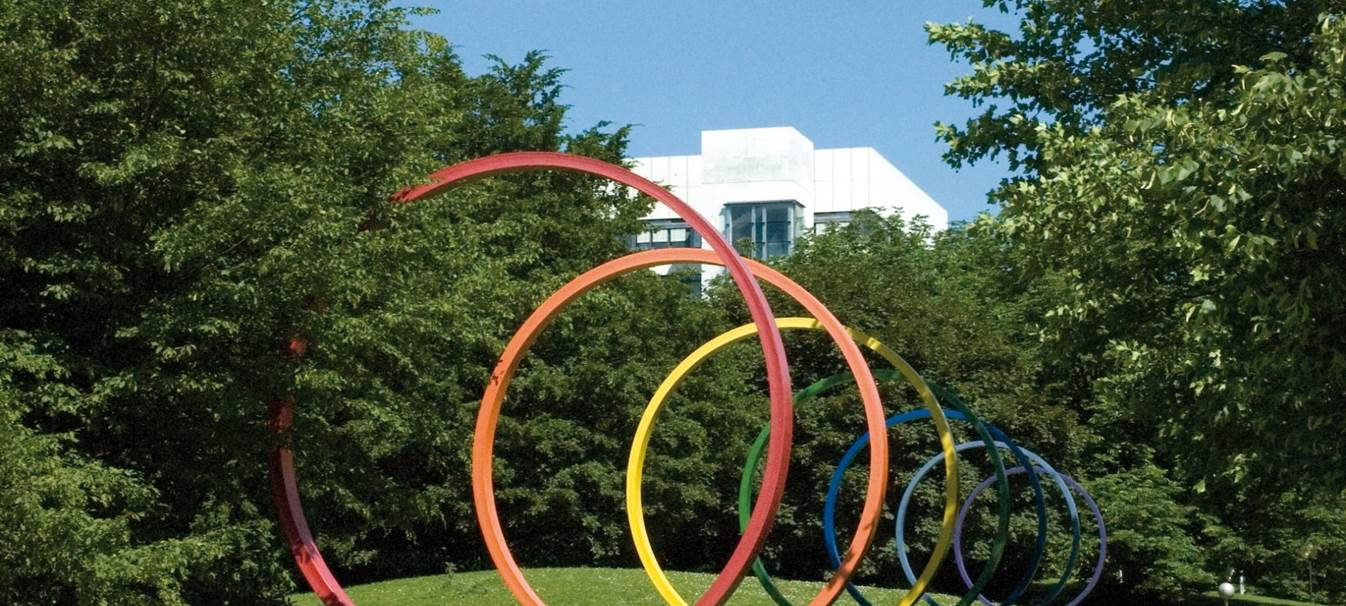
\includegraphics[width=0.7\textwidth]{images/tudo-title-2.jpg}}


\begin{document}
\maketitle
\begin{frame}
\end{frame}

\begin{frame}{Gliederung}
\begin{itemize}
  \item Stromnetz
  \begin{itemize}
  \item Vorderungen an das Stromnetz
  \item Frequenz im Netz
  \item Reguationsmechanismen der Frequenz
  \item Spannungsebenen
  \item Verteilung
  \item Netzbetreiber
  \item Anspruch an das Stromnetz durch die Energiewende
  \end{itemize}
\end{itemize}
\end{frame}
\begin{frame}
\begin{itemize}
 \item Strombörse
\begin{itemize}
  \item Enwicklung der Strombörse
  \item Angebote der Strombörse
  \item Spot Markt(und seine Folgen auf das Netz)
  \item Strompreis aus der Merit Order
  \item EEG-Umlage
  \item Strompreisentwicklung
\end{itemize}
\end{itemize}
\end{frame}



\begin{frame}{Europäisches Verbundsystem}
\end{frame}


\begin{frame}
  \begin{columns}
  \begin{column}{0.6\textwidth}
\end{column}
\begin{column}{0.4\textwidth}
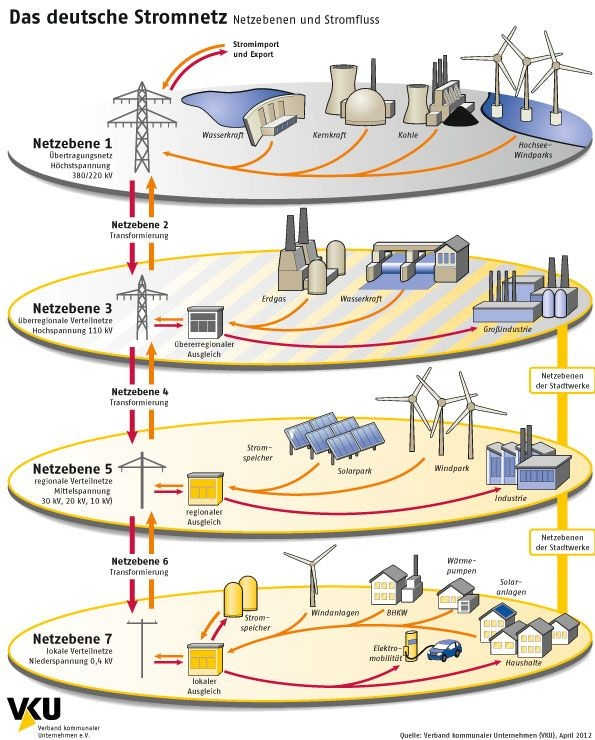
\includegraphics[width=1\textwidth]{images/netzebenen.jpg}
%Quelle: http://www.bpb.de/politik/wirtschaft/energiepolitik/148524/ausbau-des-stromnetzes
\end{column}
\end{columns}
  \begin{itemize}
    \item Höchstspannung
  \end{itemize}
\end{frame}


\begin{frame}{Netzfrequenz}
Richtfrequenz von $\SI{50}{\hertz}$ im Europäischen Verbundnetz
Abweichungen können zu Problemen wie
\begin{itemize}
  \item test ...
\end{itemize}
führen.\\
Abweichungen in der Frequenz entstehen durch Schwankungen der Relation von abgenommener und erzeugter Leistung

\end{frame}

\end{document}
